\documentclass[letterpaper, 11pt]{article}
\usepackage{amsmath}
\usepackage{amssymb}
\usepackage{float}
\usepackage{inputenc}
\usepackage[left=2cm, right=2cm, top=2cm, bottom=2cm]{geometry}
\usepackage{graphicx}
\usepackage{float}
\usepackage{caption}
\usepackage{extarrows}
\usepackage{xcolor}
\usepackage{lscape}
\usepackage{pdflscape}
\usepackage{pdfpages}
\usepackage{multicol}
\usepackage{leftindex}

\usepackage{listings}
\usepackage{color}

%Default fixed font does not support bold face
\DeclareFixedFont{\ttb}{T1}{txtt}{bx}{n}{12} % for bold
\DeclareFixedFont{\ttm}{T1}{txtt}{m}{n}{12}  % for normal

% Custom colors
\definecolor{deepblue}{rgb}{0,0,0.5}
\definecolor{deepred}{rgb}{0.6,0,0}
\definecolor{deepgreen}{rgb}{0,0.5,0}


% color def
\definecolor{darkred}{rgb}{0.6,0.0,0.0}
\definecolor{darkgreen}{rgb}{0,0.50,0}
\definecolor{lightblue}{rgb}{0.0,0.42,0.91}
\definecolor{orange}{rgb}{0.99,0.48,0.13}
\definecolor{grass}{rgb}{0.18,0.80,0.18}
\definecolor{pink}{rgb}{0.97,0.15,0.45}

% listings
% Define a custom color
\definecolor{backcolour}{rgb}{0.95,0.95,0.92}
\definecolor{codegreen}{rgb}{0,0.6,0}

% Define a custom style
\lstdefinestyle{myStyle}{
    backgroundcolor=\color{backcolour},
    commentstyle=\color{codegreen},
    basicstyle=\ttfamily\footnotesize,
    breakatwhitespace=false,
    breaklines=true,
    keepspaces=true,
    numbers=none,
    showspaces=false,
    showstringspaces=false,
    showtabs=false,
    tabsize=4,
    keywordstyle=\bfseries\color{blue},
}
\newcommand{\peq}{ \mathrel{+}= }
\newcommand{\muleq}{ \mathrel{*}= }
\newcommand{\bm}[1]{\begin{bmatrix} #1 \end{bmatrix}}
\newcommand{\lx}[2]{\leftindex #1 {#2}}
\newcommand{\norm}[1]{\left\lvert #1 \right\rvert}
\newcommand{\itbf}[1]{\textit{\textbf{#1}}}


% Use \lstset to make myStyle the global default
\lstset{style=myStyle}

\title{Problems Sets from\\Dynamics by Kane}
\author{Sesha N. Charla}
\date{\today}


\begin{document}
\maketitle
\tableofcontents
\newpage
%===============================================================================
\part{Kinematics}
\section{Problem Set 1}
%===
\subsection{1(a)}
Four rectangular parallelopipeds, A, B, C, and D, are arranged as shown in Figure~\ref{1_a}.
$\pmb a_1, \pmb a_2, \pmb a_3$ designate unit vedtors respectively parallel to the edges of $A$: $\pmb b_1, \pmb b_2, \pmb b_3$ are unit vectors respectively parallel to the edges of $B$, and so forth, and $\phi, \theta$ and $\psi$ denote the radian measures of angles that determine the relative orientiation of the bodies.
The configuration shown is one in which $\phi, \theta, \psi$ are regarded positive. Determine the maginitude of each of the following derivatives:

\begin{align*}
  \lx{^B}{\frac {\partial \pmb a_1}  {\partial \phi}}, \:
  \lx{^B}{\frac {\partial \pmb b_1}  {\partial \phi}}, \:
  \lx{^B}{\frac {\partial \pmb a_3}  {\partial \phi}}, \:
  \lx{^B}{\frac {\partial \pmb b_2}  {\partial \theta}}, \:
  \lx{^C}{\frac {\partial \pmb b_2}  {\partial \theta}}, \:
  \lx{^D}{\frac {\partial \pmb b_2}  {\partial \theta}}, \:
  \lx{^C}{\frac {\partial \pmb b_2}  {\partial \psi}}, \:
  \lx{^D}{\frac {\partial \pmb b_2}  {\partial \psi}}, \:
  \lx{^D}{\frac {\partial \pmb a_1}  {\partial \psi}}
\end{align*}

\begin{figure}[H]
    \centering
    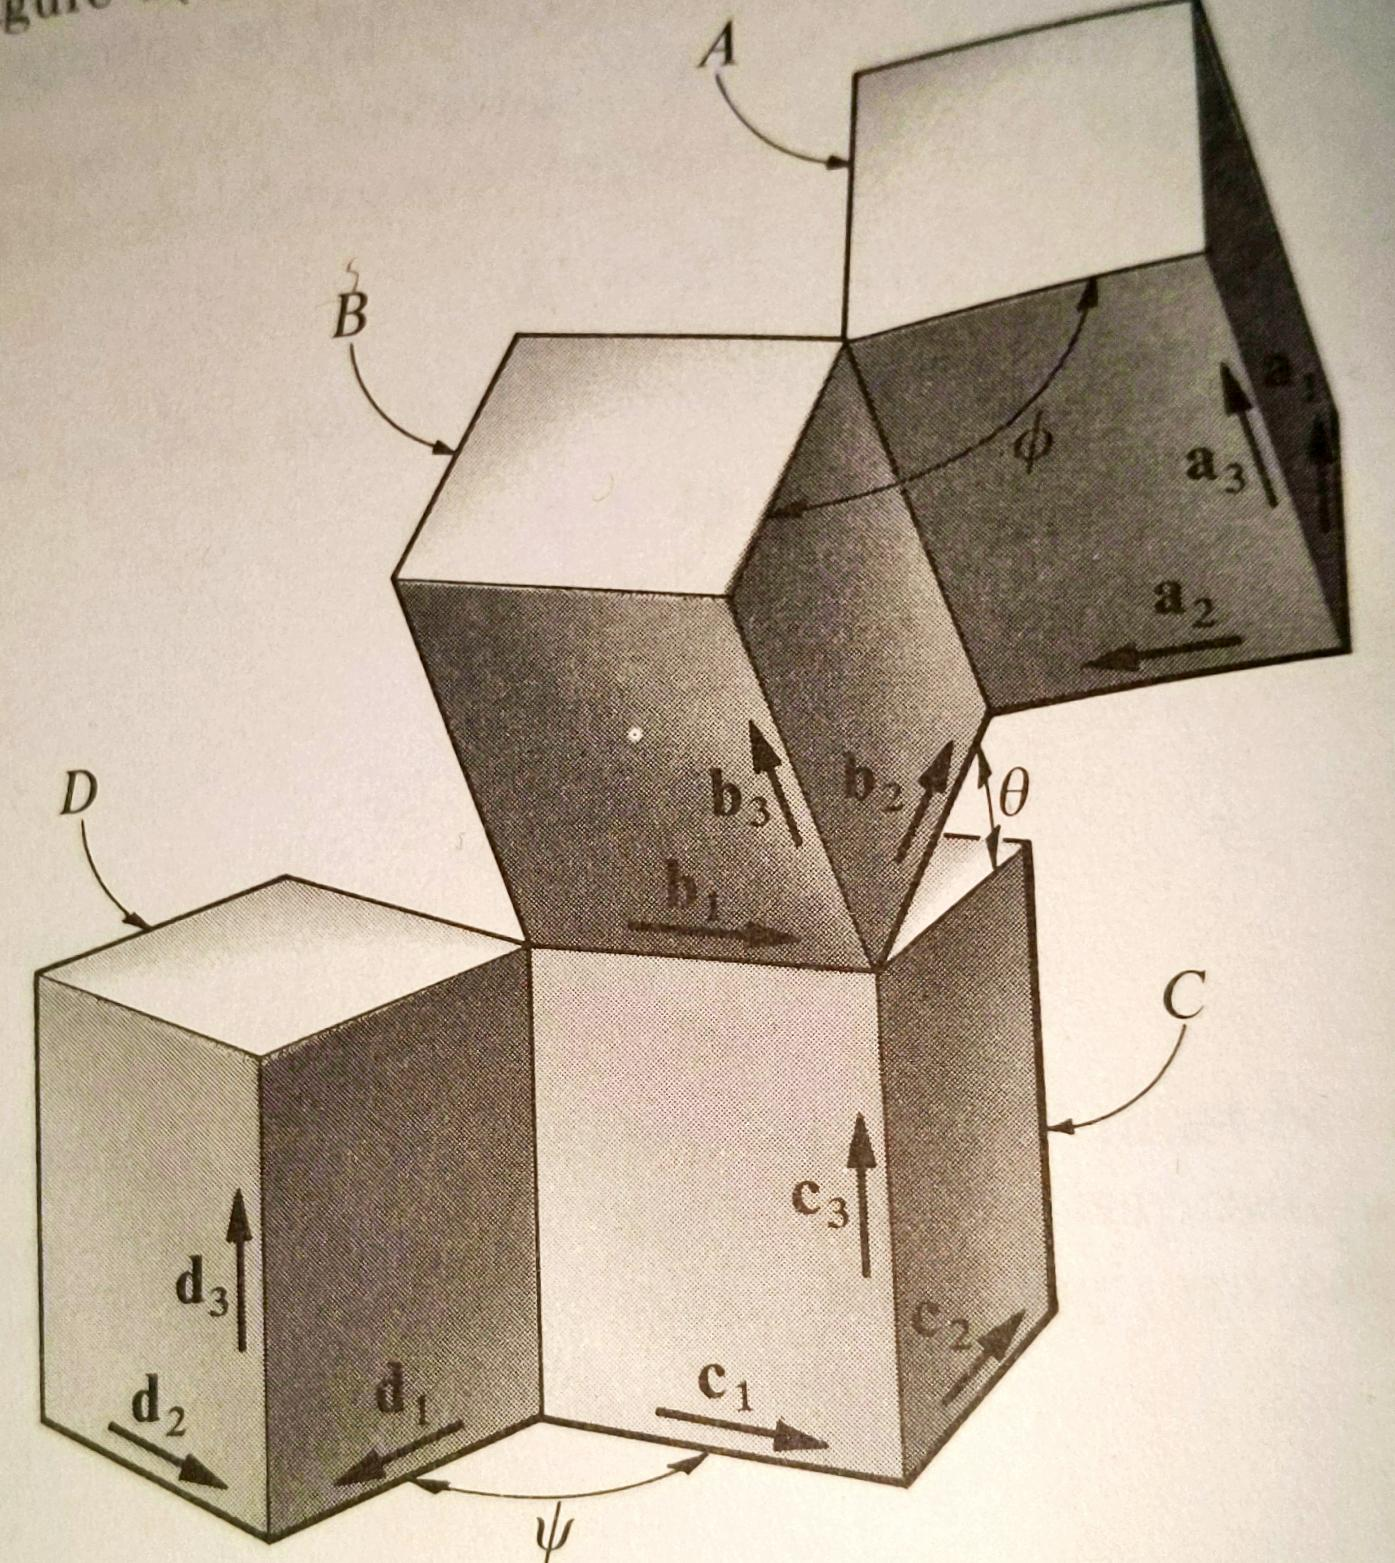
\includegraphics[width = 0.5\textwidth, height = 0.5\textwidth]{./figs/ProbSet_1/1_a.jpg}
    \caption{}
    \label{1_a}
\end{figure}


\textbf{\textit{sol.}}\\

We have the following rotation matrices:

\begin{align*}
     &\lx{^B}{\bm{\pmb a_1 \\ \pmb a_2 \\ \pmb a_3}} =
     \underbrace{
        \bm{
            \cos \phi & \sin \phi  & 0\\
            -\sin \phi & \cos \phi & 0\\
            0          & 0         & 1
        }
     } _ {R_3 (\phi)}
    \lx{^B}{\bm{\pmb b_1 \\ \pmb b_2 \\ \pmb b_3}} ;\:
    %===
    \lx{^C}{\bm{\pmb b_1 \\ \pmb b_2 \\ \pmb b_3}} =
    \underbrace{
        \bm{
            1 & 0 & 0\\
            0 & \cos \theta & \sin \theta\\
            0 & -\sin \theta & \cos \theta
        }
     } _ {R_1 (\theta)}
    \lx{^C}{\bm{\pmb c_1 \\ \pmb c_2 \\ \pmb c_3}} ;\:
    %===
    \lx{^D}{\bm{\pmb c_1 \\ \pmb c_2 \\ \pmb c_3}} =
     \underbrace{
        \bm{
            \cos \psi & \sin \psi  & 0\\
            -\sin \psi & \cos \psi & 0\\
            0          & 0         & 1
        }
     } _ {R_3 (\psi)}
    \lx{^D}{\bm{\pmb d_1 \\ \pmb d_2 \\ \pmb d_3}} \\
    %===
    &\text{Let, } \qquad
    \pmb a = \bm{\pmb a_1 \\ \pmb a_2 \\ \pmb a_3} \quad
    \pmb b = \bm{\pmb b_1 \\ \pmb b_2 \\ \pmb b_3} \quad
    \pmb c = \bm{\pmb c_1 \\ \pmb c_2 \\ \pmb c_3} \quad
    \pmb d = \bm{\pmb d_1 \\ \pmb d_2 \\ \pmb d_3}
\end{align*}

Thus, we have,

\begin{enumerate}
 \item
 \begin{align*}
   \lx{^B}{\frac {\partial \pmb a_1}  {\partial \phi}}&=
   %=
   \frac{\partial}{\partial \phi} \left(R_3(\phi)[1, :]  \times \lx{^B}{\pmb b} \right)
   %=
   = \frac{\partial R_3(\phi)[1, :]}{\partial \phi} \lx{^B}{\pmb b}
   %=
   \qquad \left[\because \pmb b_1, \pmb b_2,  \pmb b_3
   \text{ are fixed in } B \right]\\
   %=
   &= \bm{-\sin \phi & cos \phi & 0}
    \times \lx{^B}{\pmb b}\\
    %===
    &\implies \lx{^B}{\norm{\frac {\partial \pmb a_1}  {\partial \phi}}} = 1
 \end{align*}

 \item
 \begin{align*}
    \lx{^B}{\frac {\partial \pmb b_1}  {\partial \phi}} &= 0
    %=
    \implies \lx{^B}{\norm{ \frac {\partial \pmb b_1}  {\partial \phi}}} = 0
    %=
   \qquad \left[\because \pmb b_1, \pmb b_2,  \pmb b_3
   \text{ are fixed in } B \right]\\
 \end{align*}

 \item
 \begin{align*}
    \lx{^B}{\frac {\partial \pmb a_3}  {\partial \phi}} &=
   %=
   \frac{\partial}{\partial \phi} \left(R_3(\phi)[3, :]  \times \lx{^B}{\pmb b} \right)
   %=
   = \frac{\partial \pmb b_3}{\partial \phi}
   = 0
   %=
   \qquad \left[\because \pmb b_1, \pmb b_2,  \pmb b_3
   \text{ are fixed in } B \right]\\
   %===
   &\implies \lx{^B}{\norm{\frac {\partial \pmb a_3}  {\partial \phi}}} = 0
 \end{align*}


 \item
 \begin{align*}
    \lx{^B}{\frac {\partial \pmb b_2}  {\partial \theta}} &= 0
    \implies \lx{^B}{\norm{\frac {\partial \pmb b_2}  {\partial \theta}}} = 0
    \qquad \left[\because \pmb b_1, \pmb b_2,  \pmb b_3
   \text{ are fixed in } B \right]\\
 \end{align*}

\item
\begin{align*}
    \lx{^C}{\frac {\partial \pmb b_2}  {\partial \theta}} &= \frac {\partial}  {\partial \theta} \left( R_1(\theta)[2,:] \times \lx{^C}{\pmb c} \right)
    = \frac{\partial R_1(\theta)[2,:]}{\partial \theta} \times \lx{^C}{\pmb c}
    \qquad \left[\because \pmb c_1, \pmb c_2, \pmb c_3 \text{ are fixed in } C \right]\\
    %==
    &= \bm{0 & -\sin \theta & \cos \theta} \times \lx{^C}{\pmb c}\\
    %===
    &\implies \lx{^C}{\norm{\frac {\partial \pmb b_2}  {\partial \theta}}} = 1
\end{align*}


 \item
 \begin{align*}
    \lx{^D}{\frac {\partial \pmb b_2}  {\partial \theta}} &= \frac {\partial}  {\partial \theta} \left((R_1(\theta) R_3(\psi))[2,:] \times \lx{^D}{\pmb d} \right)
    \qquad \left[\because \pmb d_1, \pmb d_2, \pmb d_3 \text{ are fixed in } D \right]\\
    %===
    &= \frac{\partial (R_1(\theta) R_3(\psi))[2,:]}{\partial \theta} \lx{^D}{\bm{\pmb d_1 \\ \pmb d_2 \\ \pmb d_3}}
    %===
    = \left(\frac{\partial R_1(\theta) }{\partial \theta} R_3(\psi) \right) [2,:]\lx{^D}{\pmb d}
    %===
    = \left(\frac{\partial R_1(\theta)[2,:] }{\partial \theta} R_3(\psi) \right)\lx{^D}{\pmb d}\\
    %===
    &=  \left( \bm{0 & -\sin \theta & \cos \theta}
    \bm{
            \cos \psi & \sin \psi  & 0\\
            -\sin \psi & \cos \psi & 0\\
            0          & 0         & 1
        } \right)\lx{^D}{\pmb d}
    %===
    = \bm{\sin \theta \sin \psi & -\sin \theta \cos \psi & \cos \theta} \lx{^D}{\pmb d}\\
    %===
    &\implies  \lx{^D}{\norm{\frac {\partial \pmb b_2}  {\partial \theta}}} = 1
 \end{align*}

 \item
\begin{align*}
    \lx{^C}{\frac {\partial \pmb b_2}  {\partial \psi}} &= 0
    \implies \lx{^C}{\norm{\frac {\partial \pmb b_2}  {\partial \psi}}} = 0
    \qquad \left[ \because \text{Any vector defined in C is independent of } \psi \right]
\end{align*}

 \item
\begin{align*}
    \lx{^D}{\frac {\partial \pmb b_2}  {\partial \psi}} &= \frac{\partial}{\partial \psi} \left((R_1(\theta) R_3(\psi))[2,:] \times \lx{^D}{\pmb d} \right)
    \qquad \left[\because \pmb d_1, \pmb d_2, \pmb d_3 \text{ are fixed in } D \right]\\
    %==
    &= R_1(\theta)[2,:] \times \frac{\partial R_3(\psi)}{\partial \psi} \times \lx{^D}{\pmb d}
    %==
    = \bm{0 & \cos \theta & \sin \theta} \bm{-\sin \psi & \cos \psi & 0 \\
                                             -\cos \psi & -\sin \psi & 0\\
                                             0 & 0 & 0}
                        \times \lx{^D}{\pmb d}\\
    %==
    &= \bm{-\cos \theta \cos \psi & -\cos \theta \sin \psi & 0} \times \lx{^D}{\pmb d}\\
    %==
    &\implies  \lx{^D}{\norm{\frac {\partial \pmb b_2}  {\partial \psi}}} = \norm{\cos \theta}
\end{align*}

\item
\begin{align*}
    \lx{^D}{\frac {\partial \pmb a_1}  {\partial \psi}} &=  \frac{\partial}{\partial \psi} \left((R_3(\phi)R_1(\theta) R_3(\psi))[2,:] \times \lx{^D}{\pmb d} \right)
    %==
    = R_3(\phi)[1,:] \times R_1(\theta) \times \frac{\partial R_3(\psi)}{\partial \psi} \times \lx{^D}{\pmb d}\\
    %==
    %\quad \left[\because \pmb d_1, \pmb d_2, \pmb d_3 \text{ are fixed in } D \right]\\
    %==
    &= \bm{\cos \phi & \sin \phi  & 0}
      \bm{
            1 & 0 & 0\\
            0 & \cos \theta & \sin \theta\\
            0 & -\sin \theta & \cos \theta
        }
      \bm{
            -\sin \psi & \cos \psi  & 0\\
            -\cos \psi & -\sin \psi & 0\\
            0          & 0         & 0
        }\lx{^D}{\pmb d}\\
    %==
    &= \bm{-\cos \phi \sin \psi - \sin \phi \cos \theta \cos \psi &
          \cos \phi \cos \psi - \sin \phi \cos \theta \sin \psi &
          0} \lx{^D}{\pmb d}\\
    %==
     \implies \lx{^D}{\norm{\frac {\partial \pmb a_1}  {\partial \psi}}} &=
    \sqrt{(-\cos \phi \sin \psi - \sin \phi \cos \theta \cos \psi )^2 +
    (\cos \phi \cos \psi - \sin \phi \cos \theta \sin \psi )^2}\\
    %==
    &= (\cos^2 \phi + \sin^2\phi \sin^2 \theta)^{1/2}
\end{align*}

\end{enumerate}

\subsection{1(b)}
\textbf{\textit{Problem}}: Referring to Problem $1(a)$, determine $w_1, w_2$ and  $w_3$ such that
$$ \lx{^C}{\frac{\partial \pmb a_1}{\partial \theta}} = w_1 \pmb a_1 + w_2 \pmb a_2 + w_3 \pmb a_3$$

\textbf{\textit{sol.}}

We have,
\begin{align*}
    \lx{^C}{\frac{\partial \pmb a_1}{\partial \theta}}  &=
    \frac{\partial}{\partial \theta} [R_3(\phi)[1,:]R_1(\theta)] \times \lx{^C}{\pmb c}
    %==
    = R_3(\phi)[1,:] \frac{\partial R_1(\theta)}{\partial \theta} \times \lx{^C}{\pmb c}
    %===
    = R_3(\phi)[1,:] \frac{\partial R_1(\theta)}{\partial \theta} \times [R_3(\phi)R_1(\theta)]^{-1} \times \lx{^C}{\pmb a}\\
    %==
    &=R_3(\phi)[1,:] \frac{\partial R_1(\theta)}{\partial \theta} \times R_1^T(\theta) R_3^T(\phi)\times \lx{^C}{\pmb a}
    %==
    \qquad \left[ \because R_i^{-1} = R_i^T \right]\\
    %==
    &= \bm{\cos \phi & \sin \phi  & 0}
    \bm{
            0 & 0 & 0\\
            0 & -\sin \theta & \cos \theta\\
            0 & -\cos \theta & -\sin \theta
        }
    \bm{
            1 & 0 & 0\\
            0 & \cos \theta & -\sin \theta\\
            0 & \sin \theta & \cos \theta
    }
    \bm{
            \cos \phi & -\sin \phi  & 0\\
            \sin \phi & \cos \phi & 0\\
            0          & 0         & 1
        }
    \times \lx{^c}{\pmb a}\\
     %==
    &= \bm{\cos \phi & \sin \phi  & 0}
    \bm{
            0 & 0 & 0\\
            0 & 0 & 1\\
            0 & 1 & 0
        }
    \bm{
            \cos \phi & -\sin \phi  & 0\\
            \sin \phi & \cos \phi & 0\\
            0          & 0         & 1
        }
    \times \lx{^c}{\pmb a}
    %==
    = \bm{0 & 0 & \sin \phi} \times \lx{^c}{\pmb a}\\
    %==
    \text{Hence, }&\\
    & w_1 = w_2 = 0, \: w_3 = \sin \phi
\end{align*}

\subsection{1(c)}
\textbf{\textit{Problem}}: Referring to Problem~$1(a)$, and assuming that $\theta, \phi$ and $\psi$ are functions of the time $t$ such that, at a certain instant $t^*$, $\phi = \theta = \psi = \pi/6 \; rad$, $\dot \phi = 4 \; rad/sec$, and $\dot \theta = \dot \psi = 6 \; rad/sec$, show that at time $t^*$,
$$ \lx{^C}{\frac{\partial \pmb a_1}{\partial t}} = 4 \pmb a_2 + 3 \pmb a_3$$

\textbf{\textit{sol.}}

We have,
\begin{align*}
    \lx{^C}{{\pmb a_1}} &= R_3(\phi)[1, :] R_1(\theta) \times \lx{^C}{\pmb c}\\
    \\
    %===
    \implies \lx{^C}{\frac{d \pmb a_1}{dt}} &= \left( \frac{\partial R_3(\phi)[1, :]}{\partial \phi}   R_1(\theta) \dot \phi + R_3(\phi)[1, :] \frac{\partial R_1(\theta)}{\partial \theta } \dot \theta \right) \times \lx{^C}{\pmb c}\\
    %===
    &= \left( \frac{\partial R_3(\phi)[1, :]}{\partial \phi}   R_1(\theta) \dot \phi + R_3(\phi)[1, :] \frac{\partial R_1(\theta)}{\partial \theta } \dot \theta \right) \times R_1^T(\theta) R_3^T(\phi) \times \lx{^C}{\pmb a}\\
    %==
    &= \left[
    \left(\frac{\partial R_3(\phi)[1, :]}{\partial \phi}   R_3^T(\phi)
    \right)\dot \phi +
    \left(R_3(\phi)[1, :] \frac{\partial R_1(\theta)}{\partial \theta } R_1^T(\theta) R_3^T(\phi)
    \right) \dot \theta
    \right]\times \lx{^C}{\pmb a}\\
    %==
    &= \left[
    \left(\bm{-\sin \phi & \cos \phi & 0}\bm{
            \cos \phi & -\sin \phi  & 0\\
            \sin \phi & \cos \phi & 0\\
            0          & 0         & 1
        }
    \right)\dot \phi +
    \left(\bm{0 & 0 & \sin \phi}
    \right) \dot \theta
    \right]\times \lx{^C}{\pmb a}
    %==
    \qquad \left[\text{From } 1(b) \right]\\
    %==
    &= \left( \bm{0&1&0} \dot \phi + \bm{0 & 0 & \sin \phi} \dot \theta \right) \lx{^C}{{\pmb a}}\\
    %===
    \\
    \text{Substituting }&\; \phi = \frac{\pi}{6} \: \dot \phi =4 \; \dot \theta = 6\\
    %===
    \implies \lx{^C}{\frac{d \pmb a_1}{dt}} &= 4 \pmb a_2 + 3 \pmb a_3
\end{align*}

\subsubsection{1(d)}
\textbf{\textit{Problem}}: In Figure~\ref{1_d}, N designates a plane that is made to rotate with constant angular speed $\omega$ about a line $Z$ fixed in $N$ and in a reference frame $R$. The unit vectors $\pmb n_x, \pmb n_y$ and  $\pmb n_z$ are mutually perpendicular and fixed in R, and $\pmb n$ is a unit vector normal to $N$ and equal to $\pmb n_x$ at time $t=0$. Finally, $P_1$ and $P_2$ represent particles connected to each other by a rigid rod of lenghth $L$, these particles remaining at all times in contact with $N$.

\begin{figure}[H]
    \centering
    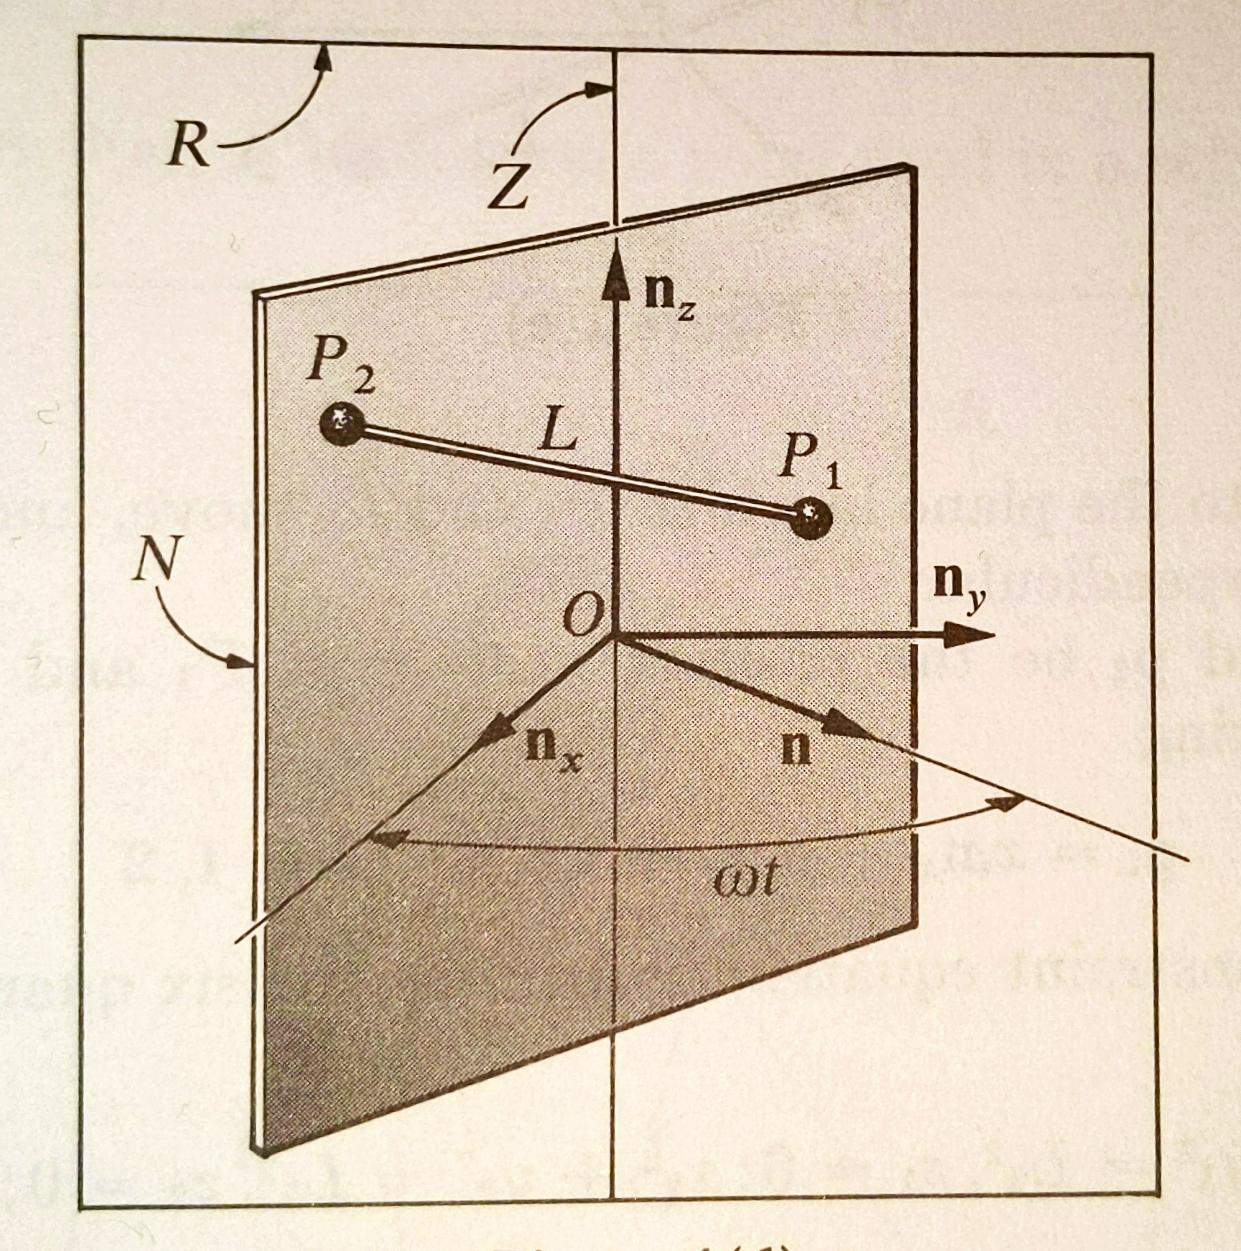
\includegraphics[width = 0.35\textwidth, height = 0.3\textwidth]{figs/ProbSet_1/1_d.jpg}
    \caption{}
    \label{1_d}
\end{figure}


Letting $\pmb p_1$ and $\pmb p_2$ be the position vectors of $P_1$ and $P_2$ relative to a point $O$ fixed in line $Z$, and taking

$$\pmb p_i = x_i \pmb n_x + y_i \pmb n_y + z_i \pmb n_z \qquad i = 1, 2$$

detarmine functions $f_j(x_1, y_1, z_1, x_2, y_2, z_2, t)$, for $j=1, 2, 3$, such that the requirements that $P_1$ and $P_2$ remain in $N$ and be separated by distance $L$ can be experessed as $f_j = 0$, $j = 1, 2, 3$.

\textbf{\textit{Sol.}}:

\begin{enumerate}
    \item For $P_1$ and $P_2$ to be attached to $N$ at all times,
    \begin{align*}
        \pmb p_i .  \pmb n &= 0 \quad \forall \; t, \qquad i = 1, 2\\
        \text{We have, } \qquad &\\
        \pmb n(t) &= \pmb n_x \sin \omega t + \pmb n_y \cos \omega t\\
        \\
        \implies \pmb p_i .  \pmb n &= x_i \sin \omega t + y_i \cos \omega t = 0 \qquad i=1, 2\\
        \\
        \therefore f_1 &= x_1 \sin \omega t + y_1 \cos \omega t\\
                   f_2 &= x_2 \sin \omega t + y_2 \cos \omega t
    \end{align*}

    \item For the distance between $P_1$ and $P_2$ to remain $L$:
    \begin{align*}
        \norm{\pmb p_1 - \pmb p_2} &= L\\
        \\
        \implies f_3 &= (x_1 - x_2)^2 + (y_1 - y_2)^2 + (z_1 - z_2)^2 - L^2
    \end{align*}
\end{enumerate}

\subsection{1(e)}

\subsection{1(f)}
\itbf{Problem}: Referring to Problem~$1(d)$, and letting S be the set of particles $P_1$ and $P_2$, determine the number of degrees of freedom of $S$ in $R$.

\itbf{Sol.}:

We have 3 constraint eqautions $(M=3)$ and 2 particles $(N=2)$. The number of degrees of freedom:
$$3N-M = 3 \times 2 - 3 = 3$$

\subsection{1(g) Generalized coordinates.}
\itbf{Problem}: Referring to the Problem~$1(e)$, express the six quantities
$x_i, y_i, z_i$ with $i=1,2$, each as a function of a single quantity $q$ in
such a way that the five constraint equations found previously are satisfied for
all values of $q$. (Suspension: Let $q$ be the radian measure of the angle
between $\pmb n_x$ and $\pmb p_2$.)

\itbf{Sol.}:

\begin{multicols}{2}
\begin{align*}
    x_1 &= -L_1 \cos q\\
    y_1 &= L_1 \sin q\\
    z_1 &=  0
\end{align*}

\begin{align*}
    x_2 &= L_2 \cos q\\
    y_2 &= -L_2 \sin q\\
    z_2 &=  0
\end{align*}
\end{multicols}

\subsection{1(h)}

\itbf{Problem}: Determine the number of degrees of freedom of each of the following holonomic systems:

\itbf{Sol.}:

\begin{enumerate}
    \item Two rigid bodies attached to each other by means of a ball-and-socket connedtion.

    --The position of both the bodies is constrained but not the orientations of the individaul bodies.
    $$n=9$$

    \item An earth satellite carrying a rotor that is made to ratate at a prescribed rate about an axis fixed in the satellite.

    -- All dof's of the rotor are constrained to that of satellite except the rotation about it's axis which is also constrained as it's rate is prescribed.
    $$n = 6$$

    \item An earth satellite carrying a rotor that is made to ratate at a prescribed rate about an axis fixed in the satellite.

    -- All dof's of the rotor are constrained to that of satellite except the rotation about it's axis.
    $$n = 7$$

    \item The particles $P_1, P_2$ of Problem~$1(e)$.

    -- The only degree of freedom is the rotation about $\pmb n_z$.
    $$n=1$$
\end{enumerate}




\end{document}
